\section{clock.h File Reference}
\label{clock_8h}\index{clock.h@{clock.h}}
{\tt \#include $<$list$>$}\par


Include dependency graph for clock.h:\nopagebreak
\begin{figure}[H]
\begin{center}
\leavevmode
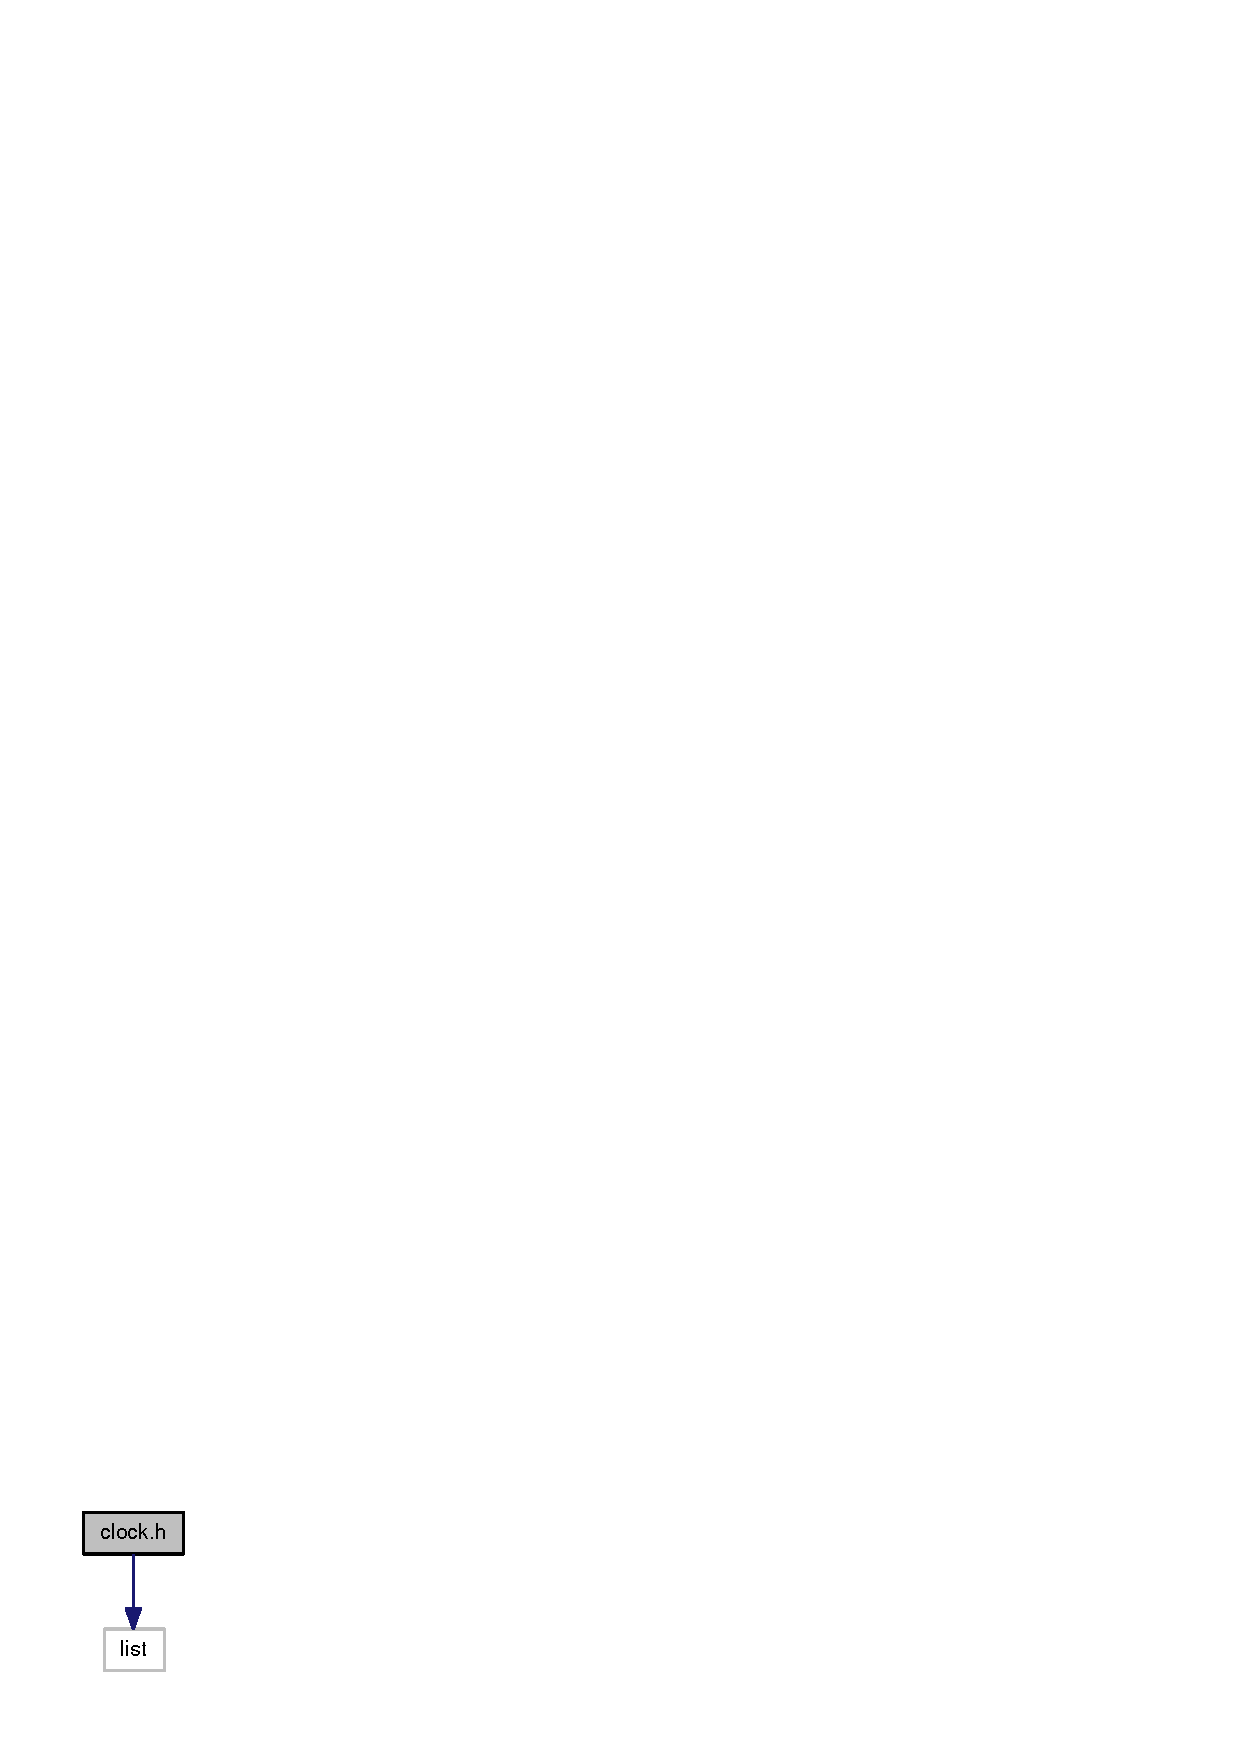
\includegraphics[width=46pt]{clock_8h__incl}
\end{center}
\end{figure}


This graph shows which files directly or indirectly include this file:\nopagebreak
\begin{figure}[H]
\begin{center}
\leavevmode
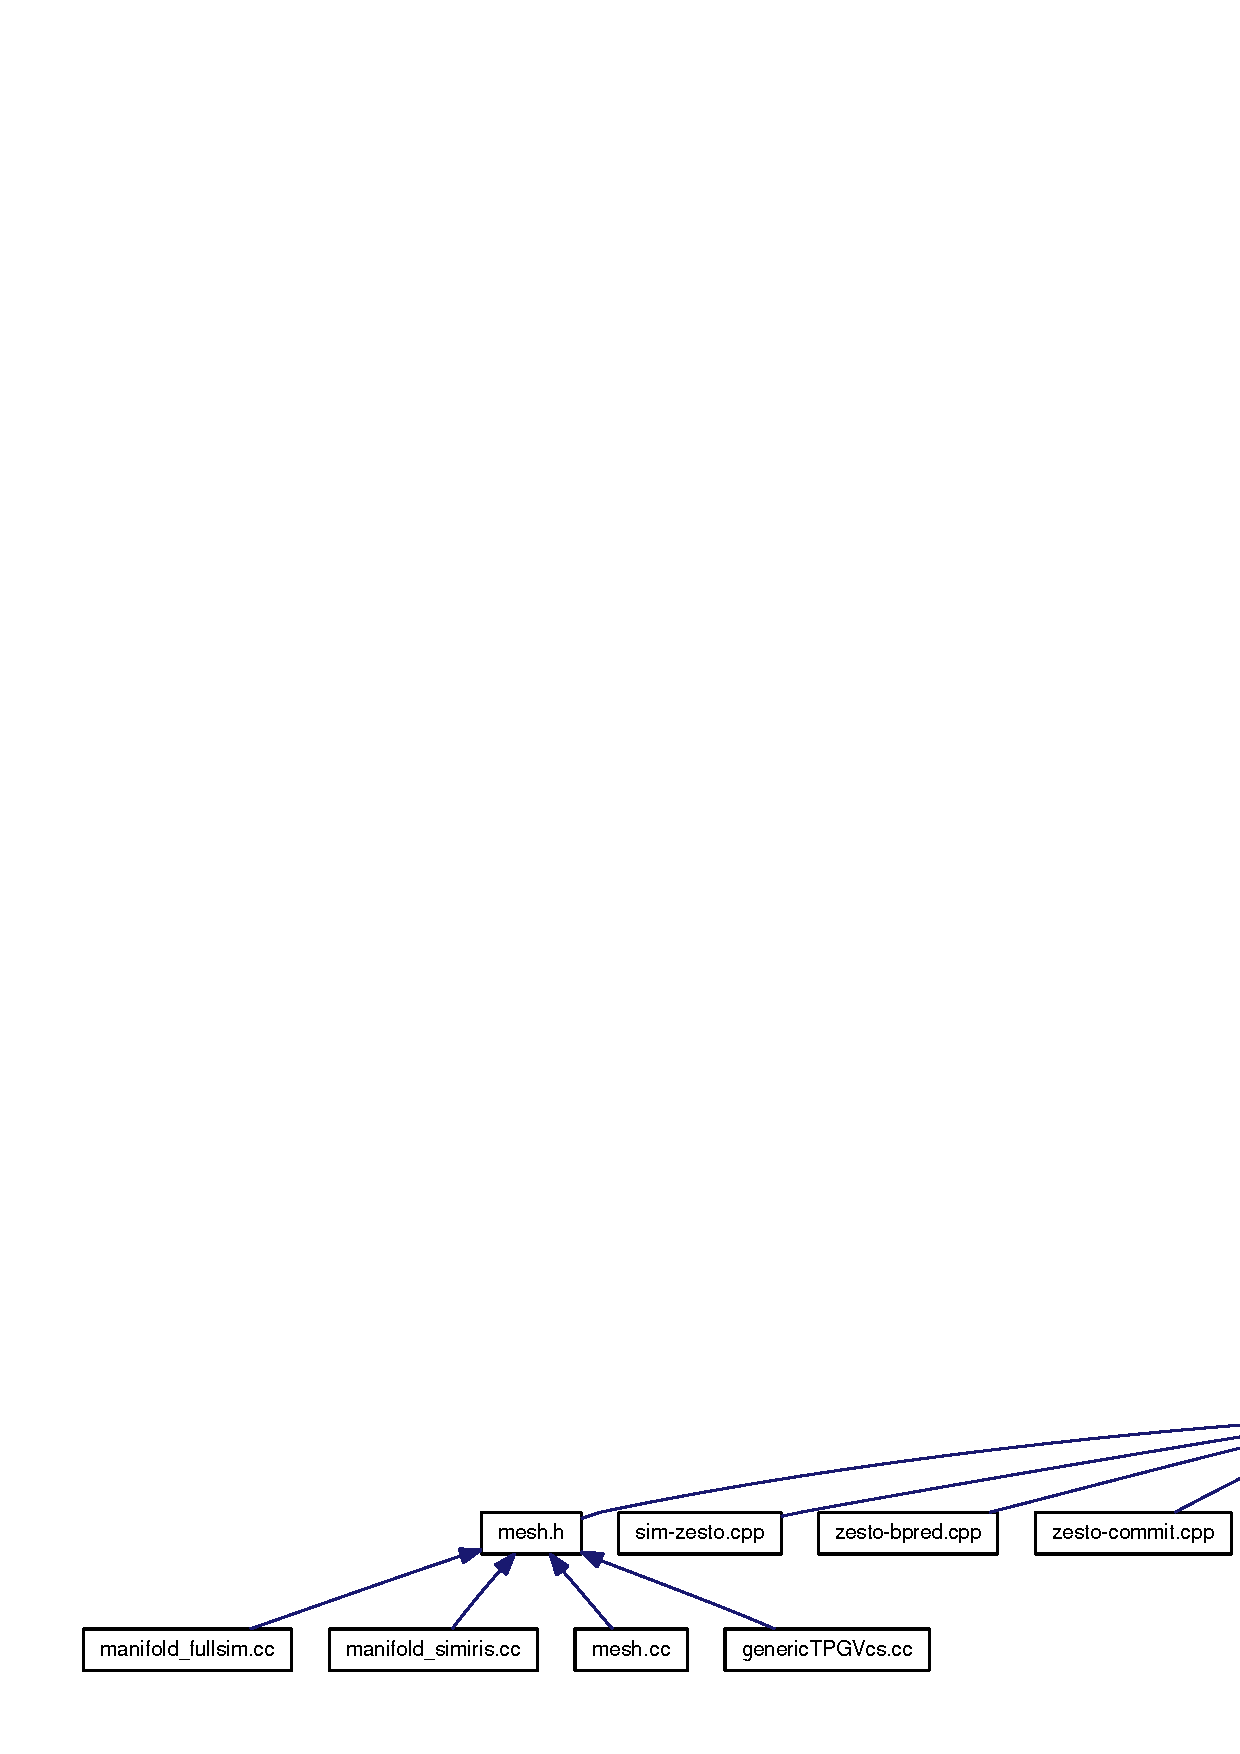
\includegraphics[width=420pt]{clock_8h__dep__incl}
\end{center}
\end{figure}
\subsection*{Classes}
\begin{CompactItemize}
\item 
class {\bf tickObjBase}
\item 
class {\bf tickObj$<$ OBJ $>$}
\item 
class {\bf Clock}
\end{CompactItemize}
\subsection*{Functions}
\begin{CompactItemize}
\item 
{\footnotesize template$<$typename OBJ $>$ }\\void {\bf registerClock} ({\bf Clock} $\ast$c, OBJ $\ast$obj, void(OBJ::$\ast$rising)(void), void(OBJ::$\ast$falling)(void))
\end{CompactItemize}


\subsection{Function Documentation}
\index{clock.h@{clock.h}!registerClock@{registerClock}}
\index{registerClock@{registerClock}!clock.h@{clock.h}}
\subsubsection[{registerClock}]{\setlength{\rightskip}{0pt plus 5cm}template$<$typename OBJ $>$ void registerClock ({\bf Clock} $\ast$ {\em c}, \/  OBJ $\ast$ {\em obj}, \/  void(OBJ::$\ast$)(void) {\em rising}, \/  void(OBJ::$\ast$)(void) {\em falling})\hspace{0.3cm}{\tt  [inline]}}\label{clock_8h_758b4082294f575c2d756c51ad23bd56}




Definition at line 38 of file clock.h.

References Clock::fallingObjs, and Clock::risingObjs.

Referenced by zesto\_\-component::zesto\_\-component().

Here is the caller graph for this function:\nopagebreak
\begin{figure}[H]
\begin{center}
\leavevmode
\includegraphics[width=203pt]{clock_8h_758b4082294f575c2d756c51ad23bd56_icgraph}
\end{center}
\end{figure}
